\documentclass[twocolumn,10pt]{article}

\usepackage[margin=0.75in,top=0.9in,bottom=0.9in,columnsep=0.25in]{geometry}
\usepackage{newtxtext,newtxmath}
\usepackage[T1]{fontenc}
\usepackage[utf8]{inputenc}
\usepackage{microtype}
\usepackage{amsmath}
\usepackage{booktabs}
\usepackage{adjustbox}
\usepackage{placeins}
\usepackage{float}
\usepackage{graphicx}
\usepackage{tikz}
\usetikzlibrary{arrows.meta,positioning,calc}
\usepackage{csquotes}
\usepackage[numbers,sort&compress]{natbib}
\usepackage{caption}
\usepackage{titlesec}
\usepackage{xcolor}
\definecolor{cvprblue}{rgb}{0.21,0.49,0.74}
\usepackage[pagebackref,colorlinks=true,linkcolor=cvprblue,citecolor=cvprblue,urlcolor=cvprblue]{hyperref}

\setcounter{topnumber}{1}
\setcounter{bottomnumber}{1}
\setcounter{dbltopnumber}{1}
\setcounter{totalnumber}{2}
\renewcommand{\topfraction}{0.8}
\renewcommand{\bottomfraction}{0.5}
\renewcommand{\dbltopfraction}{0.8}
\renewcommand{\textfraction}{0.15}
\renewcommand{\floatpagefraction}{0.85}

\captionsetup{font=small,labelsep=period,labelfont=normalfont}
\setlength{\abovecaptionskip}{4pt}
\setlength{\belowcaptionskip}{2pt}
\titleformat{\section}{\large\bfseries}{\thesection.}{0.6em}{}
\titleformat{\subsection}{\normalsize\bfseries}{\thesubsection.}{0.6em}{}
\titlespacing*{\section}{0pt}{12pt plus 2pt minus 2pt}{6pt}
\titlespacing*{\subsection}{0pt}{8pt plus 2pt minus 2pt}{4pt}
\renewcommand{\abstractname}{\normalsize\bfseries Abstract}
\renewenvironment{abstract}{\begin{center}\abstractname\end{center}\itshape\noindent\ignorespaces}{\par}
\renewcommand*{\backref}[1]{}
\renewcommand*{\backrefalt}[4]{\ifcase #1 \or #2\else #2\fi}

\title{\vspace{-1.6em}\Large\bfseries Reverse Engineering the RVQ Audio Encoder of MiniMax Music 3 via Reverse Distillation}
\author{
  \begin{tabular}{c@{\hspace{3em}}c}
    Munaza Ashraf\textsuperscript{1} & Bghira\textsuperscript{2}
  \end{tabular}\\[0.5em]
  {\small \textsuperscript{1}\href{https://github.com/MunazaAshraf10}{github.com/MunazaAshraf10}\quad
  \textsuperscript{2}\href{https://github.com/bghira/SimpleTuner}{github.com/bghira/SimpleTuner}}
}
\date{}

\begin{document}
\maketitle

\begin{abstract}
MiniMax Music 3 plans a track as eight residual vector quantised (RVQ) code streams at 25 Hz and renders them with a diffusion transformer over the latents of a continuous audio autoencoder. The encoder that maps audio back to those codes was never released, so a reference recording cannot condition the model. We learn a functional surrogate of that missing map by \emph{reverse distillation}: we generate 2,972 tracks with the model itself, keep the sampled codes together with the generator's top-50 code distributions, and train an encoder from the frozen autoencoder latents to the codes. Two design choices account for most of the result. First, the generator's code timeline is not a fixed ratio of the latent timeline but is stitched from 200-frame rollout chunks, and we recover the exact frame-to-latent correspondence and pool latents with it. Second, the acoustic codebooks are conditionally dependent across depth; replacing seven independent readouts by a decoder that is causal across codebook depth raises the downstream condition-replay cosine on 130 held-out generated tracks from 0.7698 to 0.8748 (paired bootstrap interval of the gain [0.101, 0.109]; community baseline 0.6633, true codes 0.9999) while exact-token agreement barely moves, suggesting substantial functional redundancy in the code space.

We release four encoders of 41M to 169M parameters, trained under maximal update parametrisation, together with the corpus. The recommended encoder reproduces its published token metrics to within 0.001 when re-evaluated on the same held-out split and encodes six minutes of stereo audio in 5.6 s on one RTX 3090. All evaluation is on model-generated audio and stops before the diffusion stage; calibration of the metric against random codes and a study on recorded music are the open validations.
\end{abstract}

\section{Introduction}

Codec language models generate audio as sequences of discrete codes from a neural audio codec and render those codes with a decoder~\cite{borsos2023audiolm,wang2023valle,copet2023musicgen}. MiniMax Music 3~\cite{minimax2026music3} follows this design with a twist: a Qwen3 language model~\cite{qwen3} plans one semantic codebook of 16,384 entries and an RVQ depth decoder fills in seven acoustic codebooks of 1,024 entries, eight integers per 40 ms frame, which a condition encoder turns into the conditioning of a flow-matching diffusion transformer~\cite{lipman2023flow,peebles2023dit} over 128-channel latents of a Descript-style audio autoencoder~\cite{kumar2023dac}, the DAV. The released weights cover text-to-music generation only. The component that would let audio enter the code space, an audio-to-RVQ encoder, is not released, and the released inference code contains no path that uses one.

This paper learns a functional surrogate of that component and shows, by replaying its codes through the official model, that it recovers most of the conditioning signal on the generator's own audio.\footnote{The \href{https://github.com/MunazaAshraf10/open-rvq-encoder-minimax-music3}{code} and the \href{https://huggingface.co/SimpleTuner/open-rvq-encoder-minimax-music3}{weights and corpus} are public.} Our premise is that the generator provides natural supervision for its inverse: every track it produces comes with the codes that produced it and with the generator's distribution over codes at every frame, from the language model for the semantic codebook and from the depth decoder for the acoustic ones. Encoding the waveform of such a track through the frozen DAV encoder and regressing the codes from the latents is a supervised problem with exact labels. We use the term reverse distillation descriptively for this setup: the generator supplies paired outputs and their discrete causes, and its predictive distributions provide soft targets for learning an approximate inverse mapping. It is a benign instance of the model-extraction setting in which a withheld component is recovered from query access to the released system~\cite{tramer2016stealing,carlini2024stealing}.

Three parts of the solution are of independent interest.

\paragraph{Timeline contract.} The code stream runs at 25 Hz and the latents at 86.1328125 Hz, so the nominal stride is 441/128 = 3.4453125 latents per frame. The generator, however, renders in 200-frame chunks with a 100-frame hop and stitches the latents with an integer hop of 345, and each chunk owns its frames from an offset of 25. A fixed stride therefore drifts against the true timeline by a full frame within a few chunks. We derive the exact boundary sequence, confirm it against the generator's own stitching tables, and pool latents into frames with the resulting variable spans (Sec.~\ref{sec:timeline}).

\paragraph{Causal decoding across codebook depth.} Residual codebooks are conditionally dependent: the meaning of codebook $k$ depends on which codes were chosen below it. Independent readouts show a monotone collapse of accuracy with depth. A small decoder that is autoregressive across depth, conditioned on the frame context and the codes below, removes most of the collapse under teacher forcing and lifts the downstream metric by 0.10 (Sec.~\ref{sec:depth}).

\paragraph{A downstream functional metric.} Exact agreement with the sampled code tuple is a weak proxy. Replaying predicted codes through the official language-model path and comparing the resulting condition embedding with the stored one (condition-replay cosine) separates encoders that exact-token metrics cannot: the depth decoder loses 0.32 points of free-running acoustic top-1 and gains 0.105 of replay cosine against the structurally matched encoder (Sec.~\ref{sec:results}).

Our contributions are:
\begin{itemize}
  \setlength{\itemsep}{1pt}
  \item a 2,972-track reverse-distillation corpus with sampled codes, top-50 teacher distributions and chunk stitching tables;
  \item the exact frame-to-latent timeline of MiniMax Music 3 and the pooling operator it implies;
  \item four encoders, from a 41M-parameter baseline to a 169M-parameter model with a causal depth decoder, trained under maximal update parametrisation~\cite{yang2022mup} with a hard cross-entropy plus top-50 distillation objective~\cite{hinton2015distill}, reaching 0.8748 condition-replay cosine on held-out generated tracks against a 0.6633 community baseline, with paired bootstrap intervals on every difference;
  \item evidence that downstream conditioning is substantially more tolerant to alternative code tuples than exact-token agreement suggests.
\end{itemize}

\section{Background and Related Work}

\subsection{Neural audio codecs}

Vector-quantised autoencoders~\cite{oord2017vqvae} turned audio into discrete tokens, and neural codecs made the tokens efficient: SoundStream~\cite{zeghidour2021soundstream}, EnCodec~\cite{defossez2022encodec}, HiFi-Codec~\cite{yang2023hificodec} and the Descript Audio Codec~\cite{kumar2023dac} compress waveforms with convolutional stacks descended from WaveNet~\cite{oord2016wavenet}, trained with reconstruction and adversarial losses. MiniMax Music 3's DAV follows the Descript encoder layout with the Snake activation~\cite{ziyin2020snake}, but it is a continuous variational autoencoder: its 128-channel posterior mean is the input of the diffusion transformer, and the eight discrete code streams are produced by a separate tokenizer that was not released.

\subsection{Residual vector quantisation}

Residual vector quantisation (RVQ) encodes a vector as a sum of codebook entries chosen in sequence, each codebook quantising the residual left by the previous ones~\cite{zeghidour2021soundstream}. The first codebooks carry coarse content and the later ones refine it, and the meaning of a code at depth $k$ depends on the codes chosen below it. Codec language models exploit this hierarchy with coarse-to-fine stages~\cite{borsos2023audiolm}, delayed patterns~\cite{copet2023musicgen} or a depth transformer~\cite{defossez2024moshi}. Our encoder does not learn a quantiser; it is a classifier over frozen codebooks whose entries we never observe, and Sec.~\ref{sec:analysis} shows that the conditional dependence across depth survives that framing.

\subsection{Audio tokenization for music generation}

Jukebox~\cite{dhariwal2020jukebox} modelled music with transformers over VQ-VAE codes. AudioLM~\cite{borsos2023audiolm} and MusicLM~\cite{agostinelli2023musiclm} separated semantic tokens, distilled from self-supervised speech representations such as HuBERT~\cite{hsu2021hubert}, from acoustic codec tokens. SpeechTokenizer~\cite{zhang2024speechtokenizer} and Mimi~\cite{defossez2024moshi} fold the semantic content into the first RVQ layer of the codec itself. MiniMax Music 3 uses one semantic codebook of 16,384 entries and seven acoustic codebooks of 1,024 entries, the same split, and renders the codes with latent diffusion~\cite{ho2020ddpm,lipman2023flow} over a transformer backbone~\cite{peebles2023dit,esser2024sd3}, as recent long-form music generators do~\cite{evans2024longform}.

\subsection{Existing music generation systems and model extraction}

Open music generators release their tokenizer with their language model~\cite{copet2023musicgen,agostinelli2023musiclm}; MiniMax Music 3~\cite{minimax2026music3} releases the generator but not the audio-to-code path. Recovering a model or one of its components from query access has been studied as model stealing: prediction APIs leak decision boundaries~\cite{tramer2016stealing}, black-box functionality can be copied into a knockoff network~\cite{orekondy2019knockoff}, and hidden dimensions of a production language model can be read out of its logits~\cite{carlini2024stealing}. Our problem is the benign counterpart: the released system exposes its outputs and its internal code distributions, and we recover the one component the release withholds by training on those outputs, with the temperature-scaled distillation of Hinton et al.~\cite{hinton2015distill} on the teacher's own samples~\cite{kim2016sequence,beyer2022patient}. All encoders are trained under maximal update parametrisation~\cite{yang2022mup}, and the gap we measure between teacher-forced and greedy decoding is the exposure bias of sequence models~\cite{bengio2015scheduled,ranzato2016sequence} across codebook depth rather than time.

\section{MiniMax Music 3 Audio Representation}
\label{sec:representation}

\begin{figure*}[t]
  \centering
  \resizebox{0.95\textwidth}{!}{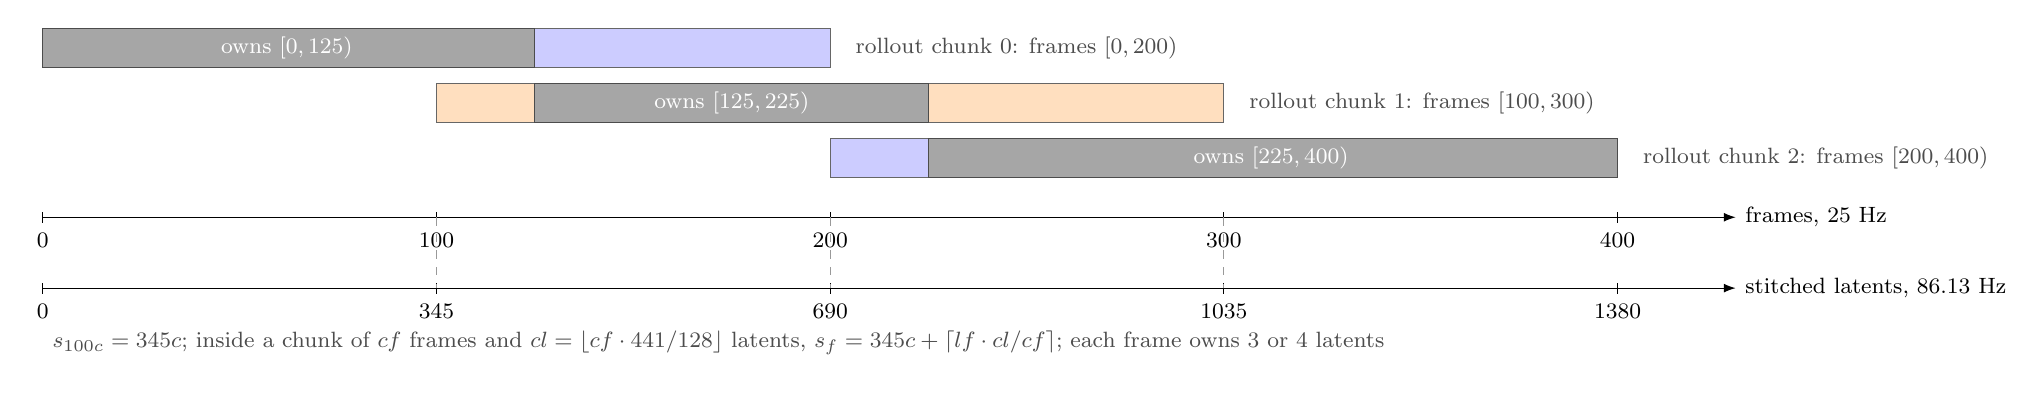
\begin{tikzpicture}[x=0.5mm,y=1mm,font=\footnotesize]
  \foreach \c/\y/\col in {0/22/blue!20,1/15/orange!25,2/8/blue!20}{
    \pgfmathtruncatemacro{\s}{\c*100}
    \pgfmathtruncatemacro{\e}{\s+200}
    \draw[fill=\col,draw=black!60] (\s,\y) rectangle (\e,\y+5);
    \node[anchor=west,text=black!70] at (\e+4,\y+2.5) {rollout chunk \c: frames $[\s,\e)$};
  }
  \draw[fill=black!35,draw=black!70] (0,22) rectangle (125,27);
  \draw[fill=black!35,draw=black!70] (125,15) rectangle (225,20);
  \draw[fill=black!35,draw=black!70] (225,8) rectangle (400,13);
  \node[text=white] at (62,24.5) {owns $[0,125)$};
  \node[text=white] at (175,17.5) {owns $[125,225)$};
  \node[text=white] at (312,10.5) {owns $[225,400)$};
  \draw[-{Latex[length=1.5mm]}] (0,3) -- (430,3) node[anchor=west]{frames, 25 Hz};
  \foreach \f in {0,100,200,300,400}{\draw (\f,2.3) -- (\f,3.7); \node[anchor=north] at (\f,2.2) {\f};}
  \draw[-{Latex[length=1.5mm]}] (0,-6) -- (430,-6) node[anchor=west]{stitched latents, 86.13 Hz};
  \foreach \f/\l in {0/0,100/345,200/690,300/1035,400/1380}{\draw (\f,-6.7) -- (\f,-5.3); \node[anchor=north] at (\f,-6.8) {\l};}
  \foreach \f in {100,200,300}{\draw[black!40,dashed] (\f,3) -- (\f,-6);}
  \node[anchor=west,text=black!70] at (0,-13) {$s_{100c} = 345c$; inside a chunk of $cf$ frames and $cl = \lfloor cf \cdot 441/128 \rfloor$ latents, $s_f = 345c + \lceil lf \cdot cl / cf \rceil$; each frame owns 3 or 4 latents};
\end{tikzpicture}
}
  \caption{The stitched timeline. Rollout chunks of 200 frames at a 100-frame hop; each chunk after the first owns its frames from local index 25; latents are stitched with a hop of 345, so a frame owns three or four latents and the boundaries follow Eq.~\ref{eq:nominal}.}
  \label{fig:timeline}
\end{figure*}

\subsection{System interface and observations}

We describe the pipeline as it can be observed from the released weights and inference code. A Qwen3-based language model~\cite{qwen3} consumes a caption and lyrics and emits, per 40 ms frame, a semantic code $c_0 \in \{0,\dots,16383\}$ or an end-of-track symbol (id 16,384). An RVQ depth decoder, a small transformer with a key-value cache over depth, emits seven acoustic codes $c_1,\dots,c_7 \in \{0,\dots,1023\}$ conditioned on the language-model hidden state and the codes below. The language model runs in windows of 200 frames with a hop of 100 frames, so every frame after the first 100 is generated twice, and the later chunk owns a frame from its local index 25 onward. A condition encoder maps the code stream to a conditioning sequence; a flow-matching diffusion transformer renders 128-channel DAV latents at 86.1328125 Hz from that conditioning, chunk by chunk, and the chunks are stitched with a hop of 345 latents; the DAV decoder returns 44.1 kHz stereo audio.

The release contains the language model, the depth decoder, the condition encoder, the diffusion transformer, and the DAV encoder and decoder. It contains neither an audio-to-code path nor the tokenizer that defines the codebooks. A reference recording therefore cannot be expressed in the code space the language model consumes.

\subsection{Initial characterisation}

Three properties of the interface shape everything that follows. The generator exposes, for every track it produces, the sampled codes and a top-50 distribution at every frame and codebook, from the language model for the semantic codebook and from the RVQ depth decoder for the seven acoustic ones, so the inverse map from audio to codes has exact labels and soft targets for free. The code stream at 25 Hz and the latent stream at 86.1328125 Hz stand in a non-integer ratio of $441/128 = 3.4453125$, and the chunked rollout with its integer stitching hop of 345 makes the true correspondence piecewise rather than a fixed stride. And the acoustic codebooks are produced by a decoder that conditions each on the codes below, so the codes of one frame are not independent labels.

\subsection{Research questions}

We ask (i) what the exact correspondence between latent and code timelines is and whether it can be reconstructed without the generator's own stitching tables; (ii) whether an encoder trained only on generated tracks can recover codes that the generator accepts as equivalent to its own; (iii) how much of the acoustic code stream can be predicted at all, given that the same audio admits many compatible code tuples; and (iv) which architectural choice, width, auxiliary alignment, or conditioning across codebook depth, moves the downstream behaviour.

\section{Reverse-Engineering Methodology}
\label{sec:methodology}


\subsection{Temporal resolution analysis}
\label{sec:timeline}

Let $n$ be the number of frames of a track. Frame $t$ covers a span $[s_t, s_{t+1})$ of stitched latents, and the $n+1$ boundaries $s_0 \le \dots \le s_n$ are the entire contract between the two timelines (Fig.~\ref{fig:timeline}).

\paragraph{Exact rule.} From the generator's stitching table, chunk 0 owns frames $[f_0, f_1 + 25)$, chunk $i > 0$ owns $[f_i + 25, f_{i+1} + 25)$, and the last chunk owns through its own end. A chunk that owns $\mathit{owned}$ frames starting at frame $g_0$ and that kept $\mathit{kept}$ latents $[a, b)$ maps its frame $g$ to $s_g = a + \lceil (g - g_0)\,\mathit{kept} / \mathit{owned} \rceil$, and a later chunk rewrites the boundary it shares with the previous one.

\paragraph{Nominal rule.} A reference recording carries no stitching table, so inference must reconstruct the timeline from the frame count alone. With $W = \max(1, \lfloor (n-1)/100 \rfloor)$ chunks, frame $f$ belongs to chunk $c = \mathrm{clamp}(\lfloor (f-25)/100 \rfloor, 0, W-1)$; a chunk of $cf = \min(200, n - 100c)$ frames yields $cl = \lfloor cf \cdot 441/128 \rfloor$ latents, and with $lf = f - 100c$,
\begin{equation}
  s_f = 345\,c + \left\lceil \frac{lf \cdot cl}{cf} \right\rceil .
  \label{eq:nominal}
\end{equation}
The rule gives $s_{100} = 345$, $s_{200} = 690$, $s_{4500} = 15{,}524$, and every span holds three or four latents; it agrees with the stitching tables on every full chunk and interpolates the shorter last chunk. A fixed stride of 3.4453125 places frame 4,500 at latent 15,504, twenty latents and almost six frames early. The 345-latent hop, the priming row and the last-chunk rule were also identified independently by a community encoder~\cite{serveurperso2026encoder}, so the contract is a property of the generator rather than of our reading of it.

\subsection{Latent representation analysis}

The DAV encoder maps 44.1 kHz audio to 1,024 channels at hop 512 and a posterior mean of 64 channels per stereo side, 128 channels at 86.1328125 Hz, left channels first. We use these posterior means, not a mel spectrogram, as the encoder input: they are the representation the diffusion transformer already consumes, and re-encoding the generated waveform through the frozen DAV encoder reproduces the generator's stored latents with 0.986 mean cosine at zero lag, so the input side of the inverse map is essentially exact. The stored flow latents themselves are not used for training because a real recording would not have them.

\subsection{Quantiser structure identification}

The observable code stream has one semantic codebook of 16,384 entries plus an end-of-track id 16,384 that never appears in audio, and seven acoustic codebooks of 1,024 entries. Row 0 of every stored code tensor is a priming row that was never emitted, so semantic frame $i$ is supervised by row $i+1$. The depth decoder that produces the acoustic codes is a two-layer causal transformer over the depth axis with a key-value cache, which fixes the direction of dependence: codebook $k$ is drawn conditioned on the language-model state and codebooks $0$ to $k-1$, never on later ones.

\subsection{Codebook analysis}

Because the codebook entries are never observed, the codebooks can only be analysed through their behaviour. Two facts emerge from training independent readouts (Sec.~\ref{sec:analysis}): top-1 agreement declines monotonically with depth, from 11 to 12\% at codebook 1 to under 3\% at codebook 7, and the same audio supports many code tuples that condition the generator identically, so exact agreement with the one sampled tuple is bounded well below the agreement that would matter downstream. Both facts point to a decoder that is conditioned across depth rather than seven independent classifiers.

\subsection{Architecture inference}

From the above we infer the shape of the missing encoder: a front end at the latent rate with a receptive field of a few frames, a pooling step that follows the stitched timeline exactly, a bidirectional context model over a window, a semantic readout, and a decoder over depth that mirrors the generator's own. Section~\ref{sec:encoder} instantiates that inference.

\section{Reconstructed Audio Encoder}
\label{sec:encoder}

We train four encoders that share one design and differ in one change each (Tab.~\ref{tab:family}). v1 is the baseline; v2 widens the shared encoder; v3 adds a training-only auxiliary objective to v2; v4 keeps the v2 encoder and replaces the independent acoustic readouts by a decoder that is causal across codebook depth. Every model is trained from scratch; no weights are transferred between versions.

\begin{table}[t]
\centering\small
\caption{The four encoders. Parameter counts are those of the released weights.}
\label{tab:family}
\adjustbox{max width=\columnwidth}{\begin{tabular}{llrr}
\toprule
Model & Change from the previous model & Width & Parameters \\
\midrule
v1 & baseline, 7 independent acoustic readouts & 512 & 40,978,944 \\
v2 & shared encoder widened, 8 to 17 heads & 1,088 & 154,736,064 \\
v3 & v2 plus training-only MERT alignment & 1,088 & 154,736,064 \\
v4 & v2 encoder plus causal depth decoder & 1,088 & 169,008,576 \\
\bottomrule
\end{tabular}}
\end{table}

\begin{figure*}[t]
  \centering
  \resizebox{0.92\textwidth}{!}{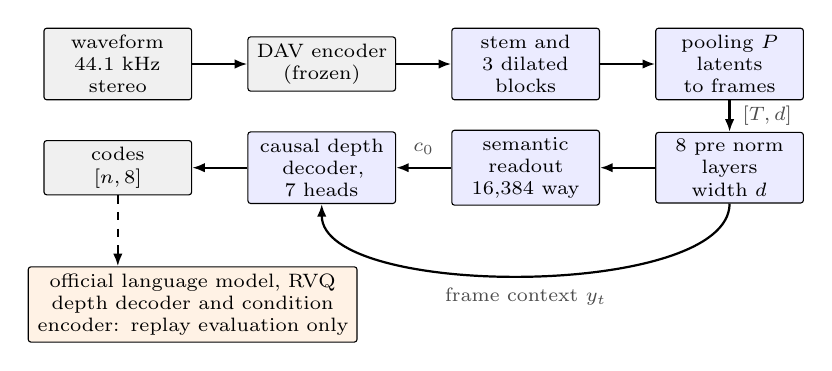
\begin{tikzpicture}[
  node distance=4mm and 7mm,
  box/.style={draw,rounded corners=1pt,align=center,font=\scriptsize,inner sep=2.5pt,minimum height=5.5mm,text width=17mm},
  frozen/.style={box,fill=black!6},
  ours/.style={box,fill=blue!8},
  official/.style={box,fill=orange!10},
  arr/.style={-{Latex[length=1.6mm]},thick},
  lab/.style={font=\scriptsize,text=black!70}
]
\node[frozen] (wav) {waveform\\44.1 kHz stereo};
\node[frozen,right=of wav] (dav) {DAV encoder\\(frozen)};
\node[ours,right=of dav] (stem) {stem and\\3 dilated blocks};
\node[ours,right=of stem] (pool) {pooling $P$\\latents to frames};
\node[ours,below=of pool] (tr) {8 pre norm layers\\width $d$};
\node[ours,left=of tr] (sem) {semantic readout\\16,384 way};
\node[ours,left=of sem] (depth) {causal depth\\decoder, 7 heads};
\node[frozen,left=of depth] (codes) {codes\\$[n, 8]$};
\draw[arr] (wav) -- (dav);
\draw[arr] (dav) -- (stem);
\draw[arr] (stem) -- (pool);
\draw[arr] (pool) -- node[lab,right=1pt]{$[T,d]$} (tr);
\draw[arr] (tr) -- (sem);
\draw[arr] (sem) -- node[lab,above=1pt]{$c_0$} (depth);
\draw[arr] (tr.south) to[out=-90,in=-90,looseness=0.6] node[lab,below=1pt]{frame context $y_t$} (depth.south);
\draw[arr] (depth) -- (codes);
\node[official,below=9mm of codes,text width=40mm,anchor=north west] at ([xshift=-2mm]codes.south west) (lm) {official language model, RVQ depth decoder and condition encoder: replay evaluation only};
\draw[arr,dashed] (codes.south) -- (lm.north -| codes.south);
\end{tikzpicture}
}
  \caption{Waveform to codes. The DAV encoder yields $[L,128]$ latents, pooling yields $[T,d]$ frame features. Grey: frozen and released components. Blue: the encoder trained here. Orange: the official path used only to compute condition-replay cosine.}
  \label{fig:pipeline}
\end{figure*}

\subsection{Architecture}

The input is the DAV posterior mean $h \in \mathbb{R}^{L \times 128}$ of a window (Fig.~\ref{fig:pipeline}). A convolutional stem (kernel 7, 128 to $d$ channels) and three residual blocks $x + \mathrm{conv}_1(\mathrm{gelu}(\mathrm{conv}_3(\mathrm{gelu}(\mathrm{GN}_1(x)))))$ with dilations 1, 3 and 9~\cite{yu2016dilated} operate at the latent rate, with GELU activations~\cite{hendrycks2016gelu}. GroupNorm with one group~\cite{wu2018groupnorm} normalises channels and time jointly, so zero-padded latents behave identically in batched and single-window evaluation. Frame features are the mean of the latent features a frame was rendered from,
\begin{equation}
  P_{t,l} = \frac{1}{s_{t+1} - s_t} \;\text{ for } l \in [s_t, s_{t+1}),\qquad 0 \text{ otherwise},
  \label{eq:pool}
\end{equation}
so every row of $P$ sums to one; $P$ maps the result to $T \le 128$ frames, learned positions are added, and eight bidirectional pre-norm transformer layers~\cite{vaswani2017attention,xiong2020prenorm} (width $d$, head dimension 64, feed-forward $4d$, dropout 0.1) followed by a LayerNorm~\cite{ba2016layernorm} give frame features $y \in \mathbb{R}^{T \times d}$. The window is 128 frames, 5.12 s, with no state across windows.

\subsection{Quantisation pipeline}
\label{sec:depth}

The semantic readout maps $y$ to 16,384 logits. v1 to v3 read the seven acoustic codebooks from $y$ with independent linear heads. v4 replaces them with a decoder that is autoregressive across codebook depth and runs once per frame: the sequence $[W_{\mathrm{ctx}} y_t,\, e_0(c_0),\, e_1(c_1),\, \dots,\, e_6(c_6)]$ plus learned depth positions passes through two causal pre-norm layers of width 512 (8 heads, feed-forward 2,048), and head $j$ reads position $j+1$ to predict codebook $j+1$. Codebook $k$ therefore sees the frame context, the semantic code and the codebooks below $k$, and nothing above. Training teacher-forces the sampled codes in one pass; inference feeds back greedy predictions in seven sequential passes, and the argmax of each head is the emitted code. The decoder adds 22.1M parameters to the 147M of the shared encoder and semantic readout.

Let $V_k$ be the size of codebook $k$. With $K = 8$ codebooks, sampled codes $c_{t,k}$, and the stored top-50 ids $i$ and teacher logits $z_T$, the objective is
\begin{align}
  \mathcal{L} &= \frac{1}{K}\sum_k \mathrm{CE}_k + w_{\mathrm{KL}} \frac{1}{K}\sum_k \mathrm{KL}_k, \label{eq:loss}\\
  \mathrm{KL}_k &= \tau^2 \sum_{i \in \mathrm{valid}} p_T(i)\big(\log p_T(i) - \log p_S(i)\big), \nonumber
\end{align}
where $p_T = \mathrm{softmax}(z_T / \tau)$ over the valid stored ids, $p_S$ is the student softmax over the whole vocabulary at temperature $\tau$ gathered at those ids, and ids outside $[0, V_k)$, notably the end-of-track id and padding, are dropped before renormalising the teacher~\cite{hinton2015distill}. All models use $w_{\mathrm{KL}} = 0.25$ and $\tau = 1$. For v4 the acoustic terms are teacher-forced, so its loss is conditional and not comparable with v1 to v3.

\subsection{Implementation}

Because each row of $P$ is one contiguous constant block, $P h$ is a segment mean and is computed in $O(L d)$ by scattering each latent into its owning frame and dividing by the span, rather than in $O(T L d)$ as a dense product. Fused scaled dot-product attention~\cite{dao2022flash,dao2024flash2,rabe2021memory} is used in the temporal stack and an unfused kernel in the depth decoder, a choice decided by measurement (Sec.~\ref{sec:results}). All models use maximal update parametrisation~\cite{yang2022mup} with width multiplier $m = d/128$: readouts compute $W(x/m) + b$, attention logits are scaled by $8/d_h$, and matrix-like weights take learning rate $\mathrm{lr}/m$ and weight decay $\mathrm{wd}\cdot m$ under AdamW~\cite{kingma2015adam,loshchilov2019adamw}; biases with a width-sized fan-in and non-zero readouts are scaled by $\sqrt{m}$ at initialisation, and the semantic readout starts at zero. The DAV encoder is evaluated in 30 s segments with 1 s margins, so peak memory is flat for any track length.

\section{Experimental Setup}
\label{sec:setup}

\subsection{Dataset}

We issued 4,000 generation requests to the released pipeline (30 flow steps, seed 20260815, 180 s requested per track, 3,772 with lyrics and 228 instrumental); 2,972 of them completed (2,775 with lyrics, 197 instrumental) and form the corpus~\cite{Bghira2026dataset}: 91.84 h of audio, mean length 1 min 51 s, with 79.6\% of tracks ending naturally on the end-of-track code. A fifth of the requests draw a deterministic sampling variant (temperature 0.85 or 1.15 with flow guidance 1.5 or 2.0); the rest use the defaults (temperature 1.0, top-50 sampling, guidance 1.5, flow guidance 1.7). Each track is stored with its audio, the sampled codes, the generator's top-50 ids and logits per frame and codebook (language model for the semantic codebook, depth decoder for the acoustic ones), the condition embeddings, the flow latents, and the chunk stitching table. A deterministic hash of the track assigns 5\% of tracks to a held-out split, so every window of a track lies in one split: 2,837 training records and 135 held-out records. The five held-out records without an exact stitching table (shards 12, 53, 73, 86 and 134) belong to the first generation batch, produced before per-chunk spans were recorded; their exclusion is determined by batch, not by content or by any failure of the encoder, and the same rule removes 178 training records. The training input is the waveform re-encoded through the frozen DAV encoder.

Table~\ref{tab:corpus} describes the content. Prompts are short genre captions, four of which (rock, pop, blues, jazz) cover 88\% of the corpus, so the held-out prompts are almost all also training prompts; lyrics are drawn from a tag-conditioned song source, and 22 of the 135 held-out tracks share their lyrics verbatim with a training track while differing in prompt, seed and sampling. The corpus is therefore narrow in caption space and the held-out split tests generalisation across generations, not across musical styles.

\begin{table}[tb]
\centering
\small
\caption{Content statistics of the reverse-distillation corpus.}
\label{tab:corpus}
\adjustbox{max width=\columnwidth}{
\begin{tabular}{lr}
\toprule
Statistic & Value \\
\midrule
tracks (train / held-out) & 2,972 (2,837 / 135) \\
with exact stitching table (train / held-out) & 2,659 / 130 \\
lyric-bearing / instrumental & 2,775 / 197 \\
distinct prompts & 307 \\
four most frequent prompts & rock (705), pop (658), blues (622), jazz (620) \\
prompt length in words, median (max) & 1 (187) \\
lyric length in lines, median (mean) & 33 (35.5) \\
held-out prompts also used in train & 124 of 135 \\
held-out lyrics identical to a training track & 22 of 135 \\
\bottomrule
\end{tabular}
}
\end{table}


\subsection{Evaluation metrics}

Evaluation uses the 130 exact-alignment held-out tracks, 2,768 deterministic 128-frame windows. \emph{Token agreement}: top-1 and top-5 inclusion of the sampled code, per codebook and pooled over the seven acoustic books; models with a depth decoder are scored free-running (greedy feedback, the inference condition) and teacher-forced. \emph{Condition-replay cosine}: the encoder's free-running codes are teacher-forced through the official language model and depth decoder, the hidden states pass through the official condition encoder with the recorded stitching, and the result is compared with the stored condition embedding, mean cosine over frames, then over tracks. True sampled codes replayed the same way score 0.9999 and are the control. The replay metric stops before the diffusion transformer; it is not a waveform or listening score, and its floor is not calibrated here: no score for random, shuffled or partially correct code tuples was available through the official path (Sec.~\ref{sec:limitations}). Every architecture was trained once, with seed 42, so differences of the order of the bootstrap intervals in Tab.~\ref{tab:bootstrap} are not interpreted.

\subsection{Baselines}

The external baseline is the community encoder of Serveurperso~\cite{serveurperso2026encoder}, a 41M model trained independently on a separate 550-track corpus with its own alignment and evaluation stack, scored under our protocol. Within our family, v1 is the size-matched baseline for that encoder and each of v2, v3 and v4 is the baseline for the next.

\subsection{Implementation details}

All runs use 4 L40S GPUs, batch 16 per rank, 20 epochs (17,660 optimizer steps), learning rate $3\times 10^{-4}$, weight decay 0.01, gradient norm clipped at 1.0, bfloat16 autocast~\cite{micikevicius2018mixed}, random 128-frame crops and seed 42. v1 used a cosine schedule of half period 500 that reheats fully every 1,000 steps~\cite{loshchilov2017sgdr}; v2 to v4 used 500 steps of linear warm-up followed by linear decay to $10^{-7}$. v3 added a training-only cosine alignment term between the layer-4 hidden state and layer 9 of a frozen MERT~\cite{li2024mert} model, weighted 0.5 until 70\% of training and annealed to zero by 90\%; its projection is not exported, so v2 and v3 share an architecture. The supplementary material (Sec.~\ref{app:hyper}) lists every hyperparameter.

\section{Results}
\label{sec:results}

\subsection{Reconstruction quality}

The quantity an encoder must reconstruct is the conditioning the generator would have received from the true codes, and Tab.~\ref{tab:replay} reports it as condition-replay cosine for every model on the 130 held-out tracks. The first column names the model and the second its parameter count; the mean is the average over tracks of the per-track cosine, the standard deviation is taken across tracks, and the 5th and 95th percentile columns bound the central ninety percent of tracks; the full range of each model is drawn in Fig.~\ref{fig:replay}. The last row is the control obtained by replaying the true sampled codes through the same path, which scores 0.9999 and marks the ceiling of the metric. Three steps are visible down the rows. The 41M baseline trained here exceeds the independent community encoder of the same size by 0.099 in mean cosine, which we attribute to the exact timeline and to the distillation term. Widening the shared encoder to 155M adds 0.007 and MERT alignment adds 0.0004, both within one standard deviation of the run before them. The causal depth decoder adds 0.105 over v3, and the whole distribution moves: its 5th-percentile track (0.845) exceeds the best track of any independent-head model (0.836), and the standard deviation shrinks from 0.019 to 0.016.

\begin{table}[tb]
\centering
\small
\caption{Condition-replay cosine on the 130 exact-alignment held-out tracks.}
\label{tab:replay}
\adjustbox{max width=\columnwidth}{
\begin{tabular}{lrrrrr}
\toprule
Model & Parameters & Mean & Std & 5th pct & 95th pct \\
\midrule
Serveurperso v1 (community) & 40,978,944 & 0.6633 & 0.0222 & 0.6281 & 0.6963 \\
v1, 41M & 40,978,944 & 0.7624 & 0.0195 & 0.7345 & 0.7904 \\
v2, 155M & 154,736,064 & 0.7698 & 0.0191 & 0.7430 & 0.7986 \\
v3, 155M + MERT & 154,736,064 & 0.7703 & 0.0193 & 0.7416 & 0.8005 \\
v4, 169M + depth & 169,008,576 & 0.8748 & 0.0157 & 0.8453 & 0.8938 \\
true codes (control) &  & 0.9999 & 0.0002 & 0.9998 & 1.0000 \\
\bottomrule
\end{tabular}
}
\end{table}


On the input side of the map, re-encoding the generated waveform through the frozen DAV encoder reproduces the generator's stored latents with 0.986 mean cosine, so the remaining gap between any model and the control is in the codes, not in the latents that feed the encoder.

Figure~\ref{fig:replay} draws the distributions of Tab.~\ref{tab:replay} as one row per model. The marker is the mean, the thick bar spans the 5th to 95th percentile, and the thin line spans the full range from the worst to the best track. Read from top to bottom, the rows step upward from the community encoder through v1, v2 and v3, whose bars overlap almost entirely, to v4, whose bar does not overlap any other model's bar; the control row sits alone at the right edge. The figure makes the two facts of the table visible at once: width and alignment move the mean by less than the width of a bar, and the depth decoder moves the entire population of tracks, not only the average.

\begin{figure}[tb]
  \centering
  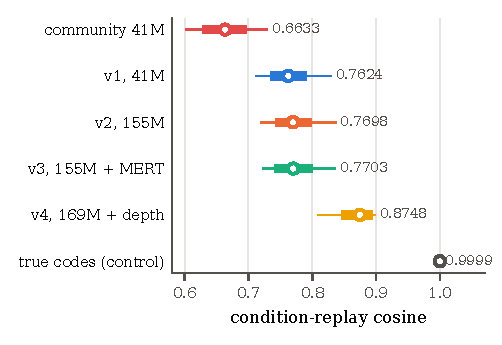
\includegraphics[width=\columnwidth]{figures/replay.pdf}
  \caption{Condition-replay cosine over the 130 held-out tracks: mean (marker), 5th to 95th percentile (bar), min to max (line). The v4 (depth-causal) distribution is separated from every independent-head model.}
  \label{fig:replay}
\end{figure}

\subsection{Token agreement}

Table~\ref{tab:matched} scores the four models on exact agreement with the sampled codes at the matched step 17,500, the last checkpoint common to all runs. The loss column is the training objective at KL weight 0.25. The four accuracy columns give top-1 and top-5 inclusion of the sampled code, first for the semantic codebook and then pooled over the seven acoustic codebooks. Semantic top-1 rises from 41.0\% to 43.2\% and semantic top-5 from 78.4\% to 80.5\% across the family, while pooled acoustic top-1 stays between 7.2\% and 7.7\% for every model; the acoustic columns are the ones that do not follow the replay metric of Tab.~\ref{tab:replay}, which is the observation Sec.~\ref{sec:analysis} builds on.

\begin{table}[tb]
\centering
\small
\caption{Exact-token metrics at the matched step 17,500 (percent).}
\label{tab:matched}
\adjustbox{max width=\columnwidth}{
\begin{tabular}{lrrrrr}
\toprule
Model & Loss & Sem. top-1 & Sem. top-5 & Ac. top-1 & Ac. top-5 \\
\midrule
v1, 41M & 5.3379 & 41.03 & 78.38 & 7.17 & 20.94 \\
v2, 155M & 5.2646 & 42.86 & 80.17 & 7.62 & 21.98 \\
v3, 155M + MERT & 5.2602 & 43.03 & 80.48 & 7.65 & 22.02 \\
v4, 169M + depth & 3.9882 & 43.16 & 80.51 & 7.30 & 19.88 \\
\bottomrule
\end{tabular}
}
\end{table}


The v4 loss is lower than the other three rows because the acoustic terms of v4 are conditioned on the true earlier codes during scoring, so they are not comparable with the independent-head rows and should not be read as a better fit. Re-evaluating the released weights on the same held-out split reproduces every published row within 0.003 in loss and 0.001 in accuracy (Sec.~\ref{app:extra}).

\subsection{Compression characteristics}

The code stream carries $14 + 7 \times 10 = 84$ bits per frame at 25 Hz, 2.1 kbit/s, against 128 latent channels at 86.13 Hz on the DAV side and 1,411 kbit/s for the 16-bit stereo waveform. The encoder is therefore a lossy map by construction, and the tolerance of the downstream conditioning to alternative tuples (Sec.~\ref{sec:analysis}) is what lets a 2.1 kbit/s stream condition the generator at 0.87 cosine. Encoding runs at 64$\times$ real time on one RTX 3090, 5.6 s for six minutes of stereo audio, four fifths of it in the frozen DAV encoder.

\subsection{Ablation studies}

Each model in Tab.~\ref{tab:family} differs from the one before it by one named change, so the rows of Tab.~\ref{tab:replay} read as an ablation, and because every model is scored on the same 130 tracks the differences are paired. Table~\ref{tab:bootstrap} gives each difference of interest with a percentile bootstrap interval: the first column names the pair, the second is the mean of the per-track differences, the third is the 95\% interval from 10,000 resamples of the 130 tracks, and the last column counts the tracks on which the first model beats the second. Three of the five comparisons improve every one of the 130 tracks: v1 over the community encoder (+0.099), v2 over v1 (+0.007) and v4 over either v2 or v3 (+0.105 and +0.1045). The MERT comparison is the exception, +0.0004 with an interval that touches zero and only 77 of 130 tracks improved, which is why we describe it as negligible for a single run rather than as an improvement.

\begin{table}[tb]
\centering
\small
\caption{Paired differences in condition-replay cosine over the same 130 tracks, with percentile bootstrap intervals (10,000 resamples).}
\label{tab:bootstrap}
\adjustbox{max width=\columnwidth}{
\begin{tabular}{lrrr}
\toprule
Comparison & Mean difference & 95\% interval & Tracks improved \\
\midrule
v1 minus community 41M & +0.0991 & [+0.0968, +0.1014] & 130 of 130 \\
v2 minus v1 & +0.0074 & [+0.0070, +0.0078] & 130 of 130 \\
v3 minus v2 & +0.0004 & [+0.0000, +0.0008] & 77 of 130 \\
v4 minus v2 & +0.1050 & [+0.1014, +0.1086] & 130 of 130 \\
v4 minus v3 & +0.1045 & [+0.1009, +0.1082] & 130 of 130 \\
\bottomrule
\end{tabular}
}
\end{table}


Two caveats limit what the ablation isolates. The larger v2 configuration improves every token metric over v1 by one to two points and replay cosine by 0.007, but v1 also used a different learning-rate schedule (a reheating cosine against linear warm-up and decay) and a different head count, so this comparison does not isolate width, and we read it only as evidence that capacity was not the main limit. MERT alignment (v2 to v3) changes token metrics by 0.03 to 0.3 points and replay by 0.0004, too little to justify a training dependency, and v4 therefore builds on the v2 encoder rather than on v3. The causal depth decoder (v4 against v2, the structurally matched comparison) improves semantic agreement marginally, \emph{lowers} free-running acoustic top-1 by 0.32 points, and raises replay cosine by 0.105, the only change that moves the downstream metric substantially. v4 also carries 22.1M more parameters than v2 in the decoder; a parameter-matched independent-head model or a non-causal decoder of the same size, which would separate conditioning from capacity, was not trained (Sec.~\ref{sec:limitations}).

Two implementation choices were also ablated by measurement. Fused attention is 3.6$\times$ faster forward and 2.8$\times$ faster backward at the temporal stack's shape (batch 16, 17 heads, length 128) and 2.9$\times$ and 3.8$\times$ slower at the depth decoder's shape (batch 2,048, 8 heads, length 8), so the two stacks use different kernels. The segment form of the pooling operator is 11$\times$ to 18$\times$ cheaper to assemble per batch than the dense matrix and equal on device (Sec.~\ref{app:extra}).

\section{Analysis}
\label{sec:analysis}

\subsection{Representation structure}

The decisive observation is the split between exact-token and downstream metrics. v4 loses 0.32 points of free-running acoustic top-1 against v2 and gains 0.105 of replay cosine; its 5th-percentile track beats the best v2 or v3 track. This suggests substantial functional redundancy in the code space: many code tuples appear to map to similar condition embeddings, and an encoder can be functionally close while disagreeing with the one tuple the generator happened to sample. Exact agreement is bounded by that sampling, not by the encoder, which is consistent with the semantic head saturating near 43\% top-1 and 80\% top-5 across every model while replay keeps improving. We have not quantified equivalence classes of tuples directly; the claim rests on the divergence of the two metrics.

Table~\ref{tab:forcing} makes the same point from inside the v4 model by scoring it under the two conditions it can be run in. Free-running, the first numeric column, is the inference condition: each acoustic head sees the greedy predictions of the heads below it. Teacher-forced, the second column, is the training condition: each head sees the sampled codes below it. The two semantic rows are identical, because the semantic readout does not depend on the acoustic codes. The two acoustic rows differ by a factor of 2.5 at top-1 (7.3\% against 18.4\%) and 2.2 at top-5 (19.9\% against 44.6\%): the decoder has learned the conditional structure of the codebooks, and feeding back its own earlier choices is what costs exact agreement. Since the replay cosine of Tab.~\ref{tab:replay} is measured on the free-running codes, the 0.8748 is achieved with the 7.3\% column, not the 18.4\% one.

\begin{table}[tb]
\centering
\small
\caption{v4 at the final checkpoint, free-running against teacher-forced (percent).}
\label{tab:forcing}
\adjustbox{max width=\columnwidth}{
\begin{tabular}{lrr}
\toprule
Metric & Free-running & Teacher-forced \\
\midrule
semantic top-1 & 43.17 & 43.17 \\
semantic top-5 & 80.51 & 80.51 \\
acoustic top-1 & 7.29 & 18.42 \\
acoustic top-5 & 19.88 & 44.55 \\
\bottomrule
\end{tabular}
}
\end{table}


\subsection{RVQ codebook behaviour}

Because the codebook entries are never observed, the codebooks can only be characterised by how predictable each one is from audio. Table~\ref{tab:depth} gives top-1 agreement for every codebook separately at the matched step 17,500. The first column is the codebook index, with 0 the semantic stream and 1 to 7 the acoustic residuals in order of depth; the next three columns are the independent-head models v1, v2 and v3; the last two are v4 free-running and v4 teacher-forced. Reading down any of the first three model columns shows the depth gradient: from 11 to 12\% at codebook 1 to under 3\% at codebook 7, and the three columns differ by at most 0.7 points at any depth. Reading down the teacher-forced column shows what the decoder learned, 27.0\% at codebook 1 and still 11.9\% at codebook 7, more than four times the independent heads at depth. The free-running column sits above v3 at codebooks 1 and 2 and falls below it from codebook 4 on, where an early disagreement has propagated through the conditioning.

\begin{table}[tb]
\centering
\small
\caption{Top-1 agreement by codebook at step 17,500 (percent).}
\label{tab:depth}
\adjustbox{max width=\columnwidth}{
\begin{tabular}{lrrrrr}
\toprule
Codebook & v1 & v2 & v3 & v4 free-running & v4 teacher-forced \\
\midrule
0 & 41.03 & 42.86 & 43.03 & 43.16 & 43.16 \\
1 & 11.27 & 11.96 & 12.04 & 14.72 & 27.04 \\
2 & 11.92 & 12.56 & 12.62 & 13.02 & 24.49 \\
3 & 9.34 & 10.00 & 9.98 & 9.46 & 19.32 \\
4 & 7.54 & 8.07 & 8.17 & 6.56 & 16.66 \\
5 & 4.45 & 4.71 & 4.74 & 3.41 & 15.46 \\
6 & 3.08 & 3.29 & 3.26 & 2.16 & 14.10 \\
7 & 2.58 & 2.77 & 2.77 & 1.76 & 11.88 \\
\bottomrule
\end{tabular}
}
\end{table}


The monotone decline of the independent heads is consistent with the conditional dependence induced by residual quantisation, where deeper codebooks refine a representation determined by the codes below and an independent head cannot see which were chosen. Under greedy feedback most of the teacher-forced gain is lost in exact agreement, the exposure bias of sequence models~\cite{bengio2015scheduled,ranzato2016sequence} across depth rather than time. The replay metric suggests that many of the alternative tuples remain functionally compatible with the generator: although they differ from the sampled tuple, they induce substantially more similar conditioning than exact-token agreement implies.

\subsection{Musical information across levels}

Figure~\ref{fig:depth} plots the seven acoustic columns of Tab.~\ref{tab:depth} against codebook index. The three solid curves of the independent-head models lie on top of one another, which is the visual form of the width and MERT ablations having no effect on the depth gradient. The dashed curve is the teacher-forced v4 decoder, the conditional structure it learned; the solid v4 curve is what survives greedy decoding, and the vertical distance between the two at each codebook is the exposure gap, widening from 12 points at codebook 1 to 10 points at codebook 7 while both curves fall. The figure also shows where the free-running v4 curve crosses below the independent heads, between codebooks 3 and 4.

\begin{figure}[tb]
  \centering
  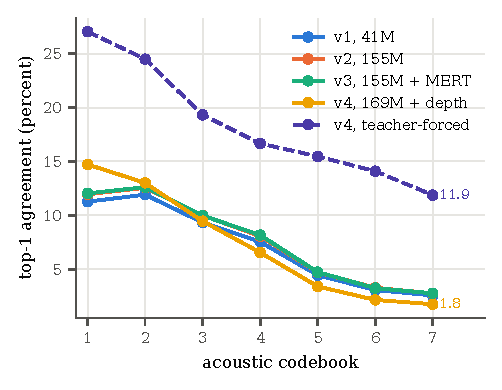
\includegraphics[width=\columnwidth]{figures/depth_gradient.pdf}
  \caption{Top-1 agreement by acoustic codebook at step 17,500. Independent heads (v1 to v3) collapse with depth; the depth-causal decoder (v4) does not when teacher-forced and partly does under greedy feedback.}
  \label{fig:depth}
\end{figure}

The semantic codebook is the most predictable stream from audio (43\% top-1, 80\% top-5 over 16,384 entries) and the one the language model plans directly; it carries the content that a text prompt determines. The acoustic codebooks refine timbre and detail and are progressively less determined by the audio alone: given the codes below, codebook 1 is predicted at 27\% and codebook 7 at 12\%, and without them the later books approach chance. Width and MERT alignment, both of which enrich the frame representation, barely move any level; conditioning across levels moves all of them. The information that matters appears to lie in the joint structure of the tuple rather than in any level in isolation.

\subsection{Implications for generative modelling}

For reference-conditioned generation the practical recipe follows from the analysis: constrain the semantic stream, which the encoder predicts well and which the language model consumes directly, and let the generator draw the acoustic codes itself. The released integration restricts every fifth generated semantic code to the encoder's top-5 candidates and generates all seven acoustic codebooks with the official depth decoder. More generally, an encoder for a hierarchical code space should be scored by what the downstream model does with its codes, and should decode across depth rather than read levels independently.

\section{Discussion}

Reverse distillation works because the generator supplies exact labels and soft targets for its own outputs, and because two structural facts about the interface, the stitched timeline and the dependence across codebook depth, can be recovered from those outputs and built into the encoder. The first fact is a matter of measurement: a fixed stride is wrong by a frame within a few chunks, and the exact rule is confirmed by the generator's own tables and by an independent implementation. The second is a matter of architecture: the same encoder features support seven independent classifiers or one causal decoder, and only the latter produces code tuples that condition the generator closely. Condition-replay cosine is the measurement that revealed this; it is cheap relative to rendering audio and stops exactly where the generator's own contribution begins. What we have shown is a functional surrogate of the withheld encoder on the generator's own distribution, not a recovery of the original component, and the surrogate's behaviour on recorded music remains to be measured.

Two results argue against natural extensions. The 3.8$\times$ larger v2 configuration moved replay cosine by 0.007, and aligning to a strong music representation moved it by 0.0004, so neither capacity nor external audio features was the limit within this family. The remaining gap to the 0.9999 control is dominated by the exposure gap of the depth decoder, and closing it is a decoding problem before it is a representation problem.

\section{Limitations and Ethical Considerations}
\label{sec:limitations}

\paragraph{Domain.} The corpus is synthetic: every training and evaluation track was generated by MiniMax Music 3 from a narrow set of genre captions, and generalisation to recorded music is not established. Anecdotally the encoder is usable on real references, but we report no metric for it.

\paragraph{Open validation.} Three measurements would bound the evidence and were not available to us, because they require the official language model, depth decoder and condition encoder as a scoring path. First, a floor for condition-replay cosine: random codes, codes from another track, and tuples with only the semantic or only the acoustic codes correct would calibrate what 0.87 means against 0.66 for the community encoder and 0.9999 for the true codes. Second, a study on recorded music, scoring functional preservation of a reference (embedding, chroma, tempo or listening judgements) after generation, since no ground-truth codes exist for real audio. Third, an end-to-end check that higher replay cosine corresponds to better preservation after the diffusion and decoding stages. Two matched ablations would sharpen the architectural claim: a 512-wide model trained with the v2 schedule, and a parameter-matched independent-head or non-causal decoder against v4.

\paragraph{Context and decoding.} The context is 128 frames (5.12 s) with no state across windows. The depth decoder has a large exposure gap between teacher-forced and greedy decoding, and we tried no beam search, scheduled sampling~\cite{bengio2015scheduled} or differentiable depth sampling. Each architecture was trained once.

\paragraph{Metrics and teacher.} Condition-replay cosine stops before the diffusion transformer and is not an audio-quality measure; exact-token agreement does not identify functionally equivalent code tuples; and the teacher distributions come from the generator's text-conditioned prior, not from an audio-conditioned posterior.

\paragraph{Ethical considerations.} No original encoder weights or source were used; the encoder is trained only on outputs of the released model, obtained through its public interface, and it does not reproduce any withheld weights. It enables reference-conditioned generation, which can be used to imitate a recording's structure; the released integration constrains only the semantic stream and leaves timbre to the generator, and use of the weights and of any generated audio remains subject to the MiniMax Music 3 terms. The corpus contains no recorded music. The v3 run's provenance additionally falls under the MERT license.

\section{Conclusion}

Using the recovered timeline contract and an encoder that decodes causally across codebook depth, we obtain 0.8748 condition-replay cosine on held-out model-generated tracks, compared with 0.7698 for the structurally matched independent-head encoder and 0.6633 for the evaluated community encoder. The results further show that condition replay separates models that exact-token metrics fail to separate, with the depth-causal decoder losing exact acoustic agreement while gaining 0.105 in replay. Calibrating the metric against random codes, measuring preservation on recorded music through the full generation pipeline, and closing the exposure gap of the depth decoder are the next steps.


\FloatBarrier
{\small
\bibliographystyle{plainnat}
\bibliography{refs}
}

\clearpage
\twocolumn[{
  \centering
  {\Large\bfseries Reverse Engineering the RVQ Audio Encoder of MiniMax Music 3 via Reverse Distillation\par}
  \vspace{0.4em}
  {\Large\bfseries Supplementary Material\par}
  \vspace{1.6em}
}]
\section{Architecture Details}
\label{app:params}

Per temporal layer $12d^2 + 13d$ parameters (four projections, two LayerNorms, feed-forward $4d$); stem $897d$; each residual block $4d^2 + 4d$; positions $128d$; output norm $2d$; a readout of size $V$ has $dV + V$. The v4 depth decoder: context projection $1{,}088 \times 512$, prior embeddings $16{,}384 \times 512 + 6 \times 1{,}024 \times 512$, depth positions $8 \times 512$, two layers of $12 \cdot 512^2 + 13 \cdot 512$, a norm, and seven heads of $512 \times 1{,}024 + 1{,}024$. Table~\ref{tab:params} evaluates these identities for the three widths; the totals are the parameter counts of the released weights, and the eight transformer layers hold 62\% of v1 and 67\% of v4.

\begin{table}[tb]
\centering\small
\caption{Parameter breakdown of the released encoders.}
\label{tab:params}
\adjustbox{max width=\columnwidth}{\begin{tabular}{lrrr}
\toprule
Component & v1 ($d{=}512$) & v2, v3 ($d{=}1{,}088$) & v4 \\
\midrule
stem & 459,264 & 975,936 & 975,936 \\
residual blocks & 3,151,872 & 14,217,984 & 14,217,984 \\
positions & 65,536 & 139,264 & 139,264 \\
transformer & 25,219,072 & 113,752,576 & 113,752,576 \\
output norm & 1,024 & 2,176 & 2,176 \\
readouts & 12,082,176 & 25,648,128 & 17,842,176 \\
depth decoder & 0 & 0 & 22,078,464 \\
\midrule
total & 40,978,944 & 154,736,064 & 169,008,576 \\
\bottomrule
\end{tabular}}
\end{table}

\section{Additional Experiments}
\label{app:extra}

\paragraph{Benchmarks.} Figure~\ref{fig:bench} shows the two measurements that decided the kernel choices of Sec.~\ref{sec:encoder}, taken on an NVIDIA GeForce RTX 3090 (sm\_86, 23.6 GiB), torch 2.14 on CUDA 13, bfloat16 autocast, tf32 enabled, with latency as the median device time over repetitions. Top: at the temporal stack's shape the fused kernel is 3.6$\times$ faster forward and 2.8$\times$ faster backward, and at the depth decoder's shape it is 2.9x and 3.8$\times$ slower, because a sequence of length 8 is below the tile size of the fused kernels and their set-up dominates. Bottom: assembling the pooling operator for a batch on the host costs 152.9 ms as dense matrices and 8.5 ms as segment indices at batch 64, and 19.8 ms against 1.8 ms at batch 16.

\begin{figure}[tb]
  \centering
  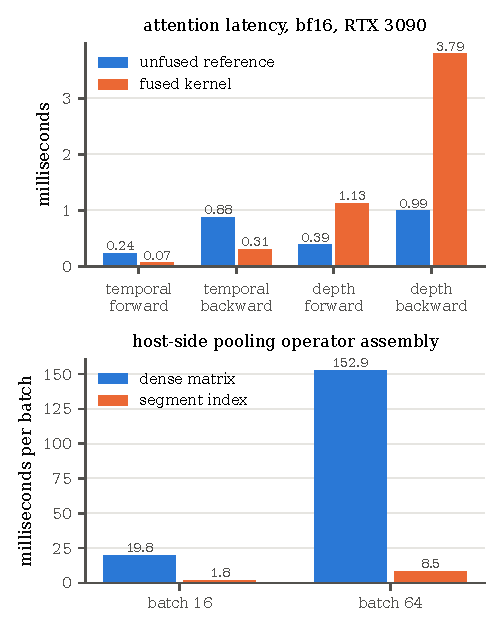
\includegraphics[width=\columnwidth]{figures/benchmarks.pdf}
  \caption{Top: attention latency at the two shapes the model runs; the fused kernel wins on the temporal stack and loses on the depth decoder. Bottom: host-side assembly of the pooling operator per batch, dense matrix against segment index.}
  \label{fig:bench}
\end{figure}

\paragraph{Held-out metrics over training.} Figure~\ref{fig:checkpoints} scores all 36 checkpoints of each run on the full held-out split. Semantic top-1 (first panel) climbs steeply for 4,000 steps and then slowly; the three wide models track one another and the 41M model runs two points below them throughout. Acoustic top-1 (second panel) shows the same ordering for the free-running curves, while the dashed teacher-forced v4 curve keeps rising to 18\% and opens the exposure gap steadily from the first checkpoint on. The held-out loss of the independent-head models (third panel) is directly comparable across v1 to v3; the v4 loss (fourth panel) is conditional on the true earlier codes and is drawn on its own axis. All curves are still improving at 17,660 steps.

\begin{figure}[tb]
  \centering
  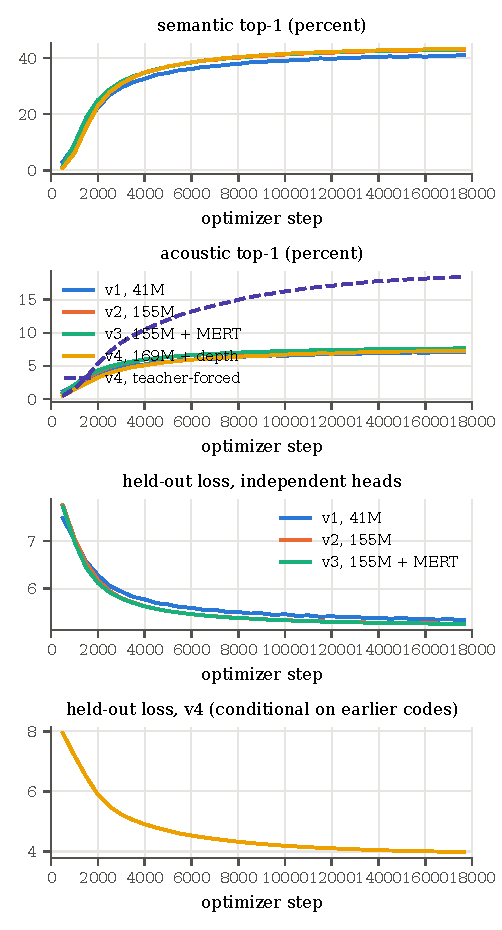
\includegraphics[width=\columnwidth]{figures/checkpoints.pdf}
  \caption{Held-out metrics over the checkpoints of every run: semantic top-1, acoustic top-1, held-out loss of the independent-head models, and the v4 loss, which is conditional on the true earlier codes and has its own panel.}
  \label{fig:checkpoints}
\end{figure}

\paragraph{Training dynamics.} Figure~\ref{fig:history} shows the training loss (top) as a running mean over 15 logged steps and the learning rate of the width-scaled parameter group relative to its peak (bottom). The loss curves order as the held-out curves do, with v4 lower because its objective is conditional. The learning-rate panel makes the schedule difference between the runs explicit: v1 follows a cosine of half period 500 that returns to its peak every 1,000 steps, whereas v2 to v4 warm up for 500 steps and decay linearly to $10^{-7}$; the v1 loss shows no visible ripple at the reheating points.

\begin{figure}[tb]
  \centering
  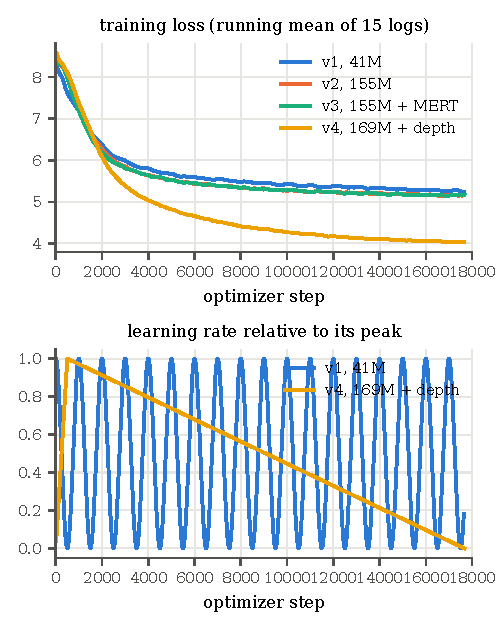
\includegraphics[width=\columnwidth]{figures/history.pdf}
  \caption{Training loss (top) and learning rate of the width-scaled parameter group relative to its peak (bottom): the v1 cosine schedule reheats every 1,000 steps, v2 to v4 warm up for 500 steps and decay linearly.}
  \label{fig:history}
\end{figure}

\paragraph{Packaged checkpoints.} v2 to v4 ship their final checkpoint at step 17,660; their held-out metrics are the published rows of Tab.~\ref{tab:reproduced}. v1 ships step 17,500 (loss 5.3379, semantic top-1 41.03\%, acoustic top-1 7.17\%), the best of its run by loss and top-1; its final checkpoint at step 17,640 is 0.003 worse in loss, a consequence of the cosine schedule ending mid-cycle. The v1 replay cosine in Tab.~\ref{tab:replay} was measured on the final checkpoint and the packaged one differs from it by 140 optimizer steps.

\paragraph{Reproducibility.} Table~\ref{tab:reproduced} places each published held-out row beside the row obtained by re-evaluating the released weights on one RTX 3090, from latents recomputed from the held-out audio. The loader yields the same 135 held-out records, 130 exact, and 2,768 windows. Every published row is reproduced within 0.003 in loss and 0.001 in accuracy under bfloat16 autocast, the teacher-forced column included, and the full float32 row for v4 moves by a further 0.001; the residual differences are float reassociation across kernels and ranks.

\begin{table}[tb]
\centering
\small
\caption{Published rows against our implementation on the same held-out split.}
\label{tab:reproduced}
\adjustbox{max width=\columnwidth}{
\begin{tabular}{lrrrrrrr}
\toprule
Model & Source & Loss & Sem. top-1 & Sem. top-5 & Ac. top-1 & Ac. top-5 & TF ac. top-1 \\
\midrule
v1, 41M & published, bf16, 4 ranks & 5.3379 & 41.03 & 7.17 &  \\
v1, 41M & this repository, bf16, 1 GPU & 5.3353 & 41.08 & 7.18 &  \\
v2, 155M & published, bf16, 4 ranks & 5.2644 & 42.86 & 7.62 &  \\
v2, 155M & this repository, bf16, 1 GPU & 5.2644 & 42.86 & 7.62 &  \\
v3, 155M + MERT & published, bf16, 4 ranks & 5.2599 & 43.03 & 7.66 &  \\
v3, 155M + MERT & this repository, bf16, 1 GPU & 5.2574 & 43.07 & 7.67 &  \\
v4, 169M + depth & published, bf16, 4 ranks & 3.9874 & 43.17 & 7.29 & 18.42 \\
v4, 169M + depth & this repository, bf16, 1 GPU & 3.9860 & 43.24 & 7.30 & 18.44 \\
v4, 169M + depth & this repository, fp32, 1 GPU & 3.9858 & 43.26 & 7.30 & 18.44 \\
\bottomrule
\end{tabular}
}
\end{table}


\paragraph{Provenance.} Table~\ref{tab:provenance} records where each released weight file came from: the training run (a repository under SimpleTuner/open-rvq-encoder-minimax-music3) and its revision, the checkpoint that was packaged, and the leading digits of the weight file's checksum, together with the dataset revision used for every number in this paper. Replay evaluation used the official components at revision fbdf52fb, and the community checkpoint is best.pt from commit d19efe9f of minimaxmusic.cpp~\cite{serveurperso2026encoder}.

\begin{table}[tb]
\centering
\small
\caption{Release provenance.}
\label{tab:provenance}
\adjustbox{max width=\columnwidth}{
\begin{tabular}{lrrrr}
\toprule
Version & Source run & Revision & Checkpoint & Weights sha256 \\
\midrule
v1 & 41m-v1 & e9fa3bba9b5b & checkpoint-17500 & 9683ba0a719fc8f4 \\
v2 & 155m-v2 & f317d72466b9 & final & 47dfffb7a76d9558 \\
v3 & 155m-v3 & 7c525705817d & final & 356e97fea65c486a \\
v4 & 169m-v4 & b9a9165b99d1 & final & e8fa93a7db2e5a09 \\
dataset & minimax-music3-rvq-reverse-distillation & 5029b1e7f1bb & holdout &  \\
\bottomrule
\end{tabular}
}
\end{table}



\section{Hyperparameters}
\label{app:hyper}

Table~\ref{tab:hyper} lists every setting of the four runs; the values are those of the released configurations, and the rows marked with a version apply to that run only.

\begin{table}[H]
\centering\small
\caption{Training and evaluation hyperparameters shared by all runs unless noted.}
\label{tab:hyper}
\adjustbox{max width=\columnwidth}{\begin{tabular}{ll}
\toprule
Setting & Value \\
\midrule
hardware & 4 x NVIDIA L40S, PyTorch DDP \\
precision & bfloat16 autocast, tf32 matmul \\
epochs, optimizer steps & 20, 17,660 (v1: 17,640) \\
batch per rank, global & 16, 64 \\
optimizer & AdamW under $\mu$P, $\beta = (0.9, 0.999)$, $\epsilon = 10^{-8}$ \\
learning rate, weight decay & $3 \times 10^{-4}$, 0.01 \\
schedule, v1 & cosine, half period 500 steps, no warm-up \\
schedule, v2 to v4 & linear warm-up 500 steps, linear decay to $10^{-7}$ \\
gradient norm limit & 1.0 \\
$\mu$P base width, multiplier & 128; 4 (v1), 8.5 (v2 to v4) \\
attention scale & $8 / d_h$, $d_h = 64$ \\
dropout & 0.1 \\
window, stride & 128 frames, random crop (train), 128 (validation) \\
KL weight, temperature, top-$k$ & 0.25, 1.0, 50 \\
MERT term, v3 only & layer 4 to teacher layer 9, weight 0.5 to 0.7 $T$, zero by 0.9 $T$ \\
depth decoder, v4 only & width 512, 2 layers, 8 heads, feed-forward 2,048 \\
validation, checkpoint interval & 500 steps \\
seed & 42 \\
\bottomrule
\end{tabular}}
\end{table}


\section{Audio Examples}
\label{app:audio}

Reference-conditioned generations produced with the released v4 encoder through the official integration are published with the weights: a 30 s reference constrained at every fifth semantic frame, and a full-length reference constrained at every fifth and at every tenth frame, each rendered as 44.1 kHz stereo. The examples use the top-5 semantic candidates of the encoder; the acoustic codebooks are generated by MiniMax Music 3 and are not copied from the reference.


\end{document}
